
\chapter{SOLUTION}
\label{chapter:Solution}

% breadth-first explanation, examples inside protocol, explain only in context of Tor

% relative vs against

\section{Overview}

We propose the Onion Name Service, or OnioNS, a system which uses enables transparent translation of .tor domain names to .onion addresses. The system has three main aspects: the generation of self-signed claims on domain names by hidden service operators, the processing of domain information within the OnioNS servers, and the receiving and authentication of domain names by a Tor client.

First, a hidden service operator, Bob, generates an association claim between a meaningful domain name and a .onion address. Without loss of generality, let this be example.tor $ \rightarrow $ example0uyw6wgve.onion. For security reasons we do not introduce a central repository and authority from which Bob can purchase domain names; however, domains are not trivially obtainable and Bob must expend effort to claim and maintain ownership of example.tor. We achieve this through a proof-of-work scheme. Proof-of-work systems are noteworthy for their asymmetry: they require the issuer to spend effort to find an answer to a moderately hard computational problem, but once solved can be easily verified correct by any recipient. The requirement of proof-of-work fulfils three main purposes:

\begin{enumerate}
	\item Significantly reduces the threat of record flooding.
	\item Introduces a barrier-of-entry that encourages the utilization of domain names and the availability of the underlying hidden services.
	\item Increases the difficulty of domain squatting, a denial-of-service attack where a third-party claims one or more valuable domain names for the purpose of denying or selling them en masse to others. In Tor's anonymous environment, this vector is particularly prone to Sybil attacks.
\end{enumerate}

Bob then digitally signs his association and the proof-of-work with his service's private key.

Second, Bob uses a Tor circuit to anonymously transmit his association, proof-of-work, digital signature, and public key to OnioNS nodes, a subset of Tor routers. This set is deterministically derived from the volatile Tor consensus documents and is rotated periodically. The OnioNS nodes receive Bob's information, distribute it amongst themselves, and later archive it in a sequential transaction database, of which each OnioNS node holds their own copy. The nodes also digitally sign this database and distribute their signatures to the other nodes. Thus the OnioNS Tor nodes maintain a common database and have each vouched for its authenticity.

Third, a Tor client, Alice, uses a Tor client to anonymously connect to one of these OnioNS nodes and request a domain name. Without loss of generality, let this request be example.tor. Alice receives Bob's ``example.tor $ \rightarrow $ example0uyw6wgve.onion'' association, his proof-of-work, his digital signature, and his public key. Alice then verifies the proof-of-work and Bob's signature against his public key, and hashes his key to confirm the accuracy of example0uyw6wgve.onion. Alice then looks up example0uyw6wgve.onion in Tor's distributed hashtable, finds Bob's introduction point, and confirms that its knowledge of Bob's public key matches the key she received from the OnioNS nodes. Finally, she finishes the Tor hidden service protocol and begins communication with Bob. In this way, Alice can contact Bob through his chosen domain name without resorting to use lower-level hidden service addresses. The uniqueness and authenticity of the Bob's domain name is maintained by the subset of Tor nodes.

%At a high level, OnionNS' master page-chain is maintained by a randomly-selected rotating set of high-capacity Tor nodes. Other Tor nodes may mirror the page-chain, distributing the load and responsibilities across the network. The system supports a variety of command and control operations including Create, Domain Query, Onion Query, Modify, Move, Renew, and Delete.

% node vs server

% capitalize nouns that are defined

\section{Definitions}

To discuss OnioNS precisely we must first define some central terms that we will use throughout the rest of this document. We detail their exact contents in section \ref{sec:DataStructures} and how they are used throughout sections \ref{sec:BasicDesign} and \ref{sec:Protocols}.

\begin{description}
	\item[domain name] \hfill \\
		A \emph{domain name} is a case-insensitive identification string claimed by a hidden service operator. The syntax of OnioNS domain names mirrors the Internet DNS; we use a sequence of name-delimiter pairs with the .tor Top Level Domain (TLD). The TLD is a name at depth one and is preceded by names at sequentially increasing depth. The term ``domain name'' refers to the identiciation string as a whole, while ``second-level domain'' refers to the central name that is immediately followed by the TLD, as illustrated in Figure \ref{fig:sampleDomain}. Domain names point to \emph{destinations} -- other domain names with either the .tor or .onion TLD.

		\begin{figure}[htbp]
			\centering
			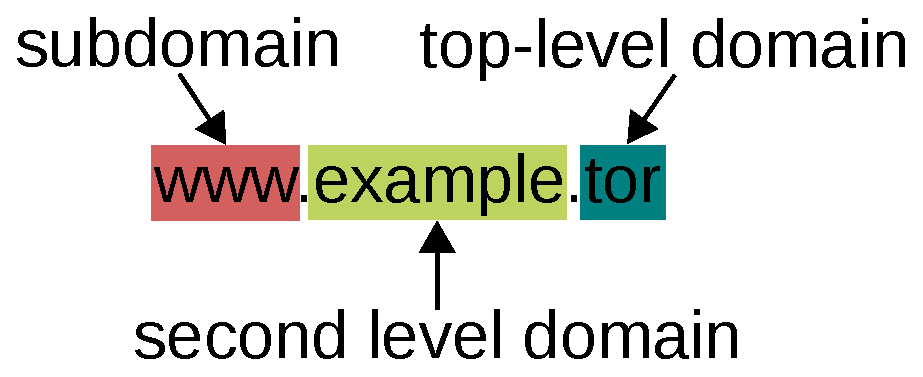
\includegraphics[width=0.5\textwidth]{images/domain-name.eps}
			\caption{A sample domain name: a sequence of labels separated by delimiters. In OnioNS, hidden service operators build associations between second-level domain names and their hidden service address.}
			\label{fig:sampleDomain}
		\end{figure}

	The Internet DNS defines a hierarchy of administrative realms that are closely tied to the depth of each name. By contrast, OnioNS makes no such distinction; we let hidden service operators claim second-level names and then control all names of greater depth under that second-level name. Hidden service operators may then choose to administer or sell the use of their subdomains, but this is outside the scope of this project.

	\item[Record] \hfill \\
		A \emph{Record} is a small textual data structure that contains one or more domain-destination pairs, a proof-of-work, a digital signature, and a public key. Records are issued by hidden service operators and sent to OnioNS servers. Every Record is self-signed with the hidden service's key. In section \ref{sec:Record} we describe the five different types of Records: Create, Modify, Move, Renew, and Delete. A Create Record represents a registration on an unclaimed second-level domain name, Modify, Move, and Renew are operations on that domain name or its subdomains, and a Delete Record relinquishes ownership over the second-level domain name and all its subdomains.

	\item[broadcast] \hfill \\
		The term for the protocol described in section \ref{sec:ProtoHiddenServices} that describes the uploading of new Records to OnioNS servers through Tor circuits and then the subsequent confirmation that the Record has been received.

	\item[Snapshot] \hfill \\
		A \emph{Snapshot} is textual database designed to hold collections of Records in a short-term volatile cache. They are also used to transmit sets of Records between OnioNS servers.

	\item[Page] \hfill \\
		A \emph{Page} is textual database designed to archive one or more Records in long-term storage. Pages are held and digitally signed by OnioNS nodes and are writable only for fixed periods of time before they are read-only. Each Page contains a link to a previous Page, forming an append-only public ledger known as an \emph{Pagechain}. This forms a two dimensional distributed data structure: the chain of Pages grows over time and there are multiple redundant copies of each Page spread out across the network at any given time.

	\item[Mirror] \hfill \\
		A \emph{Mirror} is any machine (inside or outside of the Tor network) that has performed a synchronization (section \ref{sec:Synchronization}) against the OnioNS network and now holds a complete copy of the Pagechain. Mirrors do not actively participate in the OnioNS network and do not have the power to manipulate the central page-chain.

	\item[Quorum Candidate] \hfill \\
		A \emph{Quorum Candidates} are \emph{Mirrors} inside the Tor network that have also fulfilled two additional requirements: 1) they must demonstrate that they are an up-to-date Mirror, and 2) that they have sufficient CPU and bandwidth capabilities to handle powering OnioNS in addition to their regular Tor duties. In other words, they are qualified and capable to power OnioNS, but have not yet been chosen to do so.

	\item[Quorum] \hfill \\
		A \emph{Quorum} is a subset of Quorum Candidates who have active responsibility over maintaining the master OnioNS Pagechain. Each Quorum node actively its own Page, which has a lifetime of that Quorum. The Quorum is randomly chosen from Quorum Candidates as described in section \ref{sec:ProtoTorClients}.

	\item[flood] \hfill \\
		The term for the periodic burst of communication that occurs between Quorum nodes wherein Snapshots are exchanged and each Quorum node obtains the state and digital signature of the current Page maintained by all other Quorum nodes. This communication is described in section \ref{sec:ProtoOnioNServers}.
\end{description}

\begin{figure}[htbp]
	\centering
	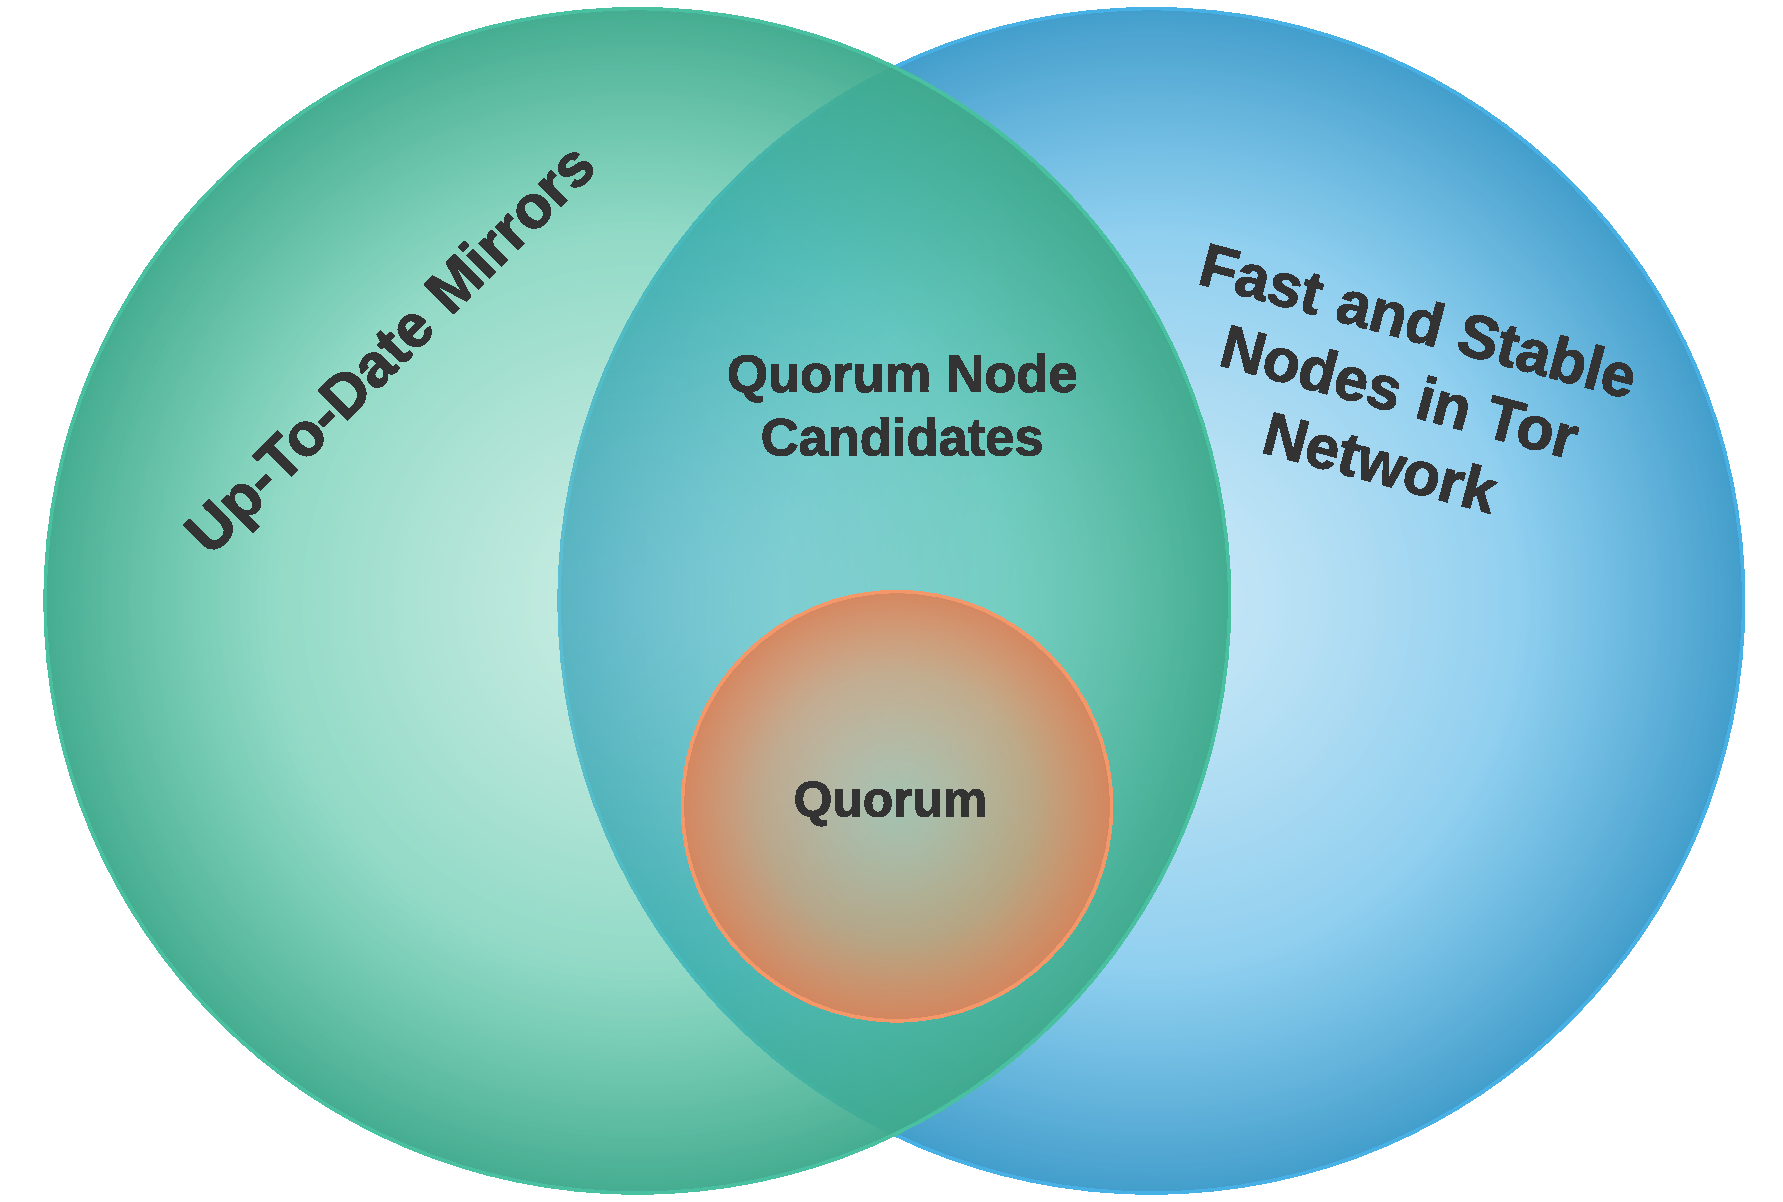
\includegraphics[width=0.5\textwidth]{images/LucidCharts/Participants.pdf}
	\caption{The relationship between Mirrors, Quorum Candidates, and the Quorum. A Mirror is any machine that holds the OnioNS Pagechain, Quorum Candidates are both up-to-date Mirrors and reliable Tor nodes, and the Quorum is randomly selected from the pool of Quorum Candidates.}
\end{figure}

Throughout the rest of this document, let Alice be a Tor client, and Bob be the operator of a hidden service. Assume that neither Alice nor Bob run Tor relays themselves, but let them only use Tor. Therefore Alice and Bob know the public keys of the Tor authority nodes and they can obtain and fully verify any past or current set of consensus documents. Bob has access to his hidden service private RSA key and may or may not have a PGP key with a subkey for email encryption.

\section{Basic Design}
\label{sec:BasicDesign}

OnioNS is build on a fundamental sequence of operations, as illustrated in Figure \ref{fig:basicDesign}:

\begin{enumerate}
	\item Bob generates a valid Record.
	\item Bob broadcasts the Record to the Quorum.
	\item The Record is flooded across the Quorum.
	\item Each Quorum node stores the Record into its current Page at the head of its local Pagechain.
	\item Alice queries the system for a domain name.
	\item Alice receives back the Record matching that domain name and confirms its validity.
	\item Alice connects to Bob via the hidden service protocol.
\end{enumerate}

These steps describe the propagation of any Record throughout the entire network. The protocols for each party are described in sections \ref{sec:ProtoHiddenServices}, \ref{sec:ProtoOnioNServers}, and \ref{sec:ProtoTorClients}, respectively. It should be noted that the activities of Alice, Bob, and the Quorum occur asynchronously: hidden service operator may be transmitting Records to the Quorum at the same time that clients are querying for other domain names.

\begin{figure}[htbp]
	\centering
	\begin{tikzpicture}[->, node distance=2.4cm, main node/.style={circle, fill=blue!20, draw, font=\sffamily\bfseries}]

			\node[main node] (1) {$ R_{G} $};
			\node[main node] (2) [right of=1] {};
			\node[main node] (3) [right of=2] {Alice};
			\node[main node] (4) [right of=3] {};

			\node[main node] (5) [below of=1] {$ R_{E} $};
			\node[main node] (6) [right of=5] {$ R_{M} $};
			\node[main node] (7) [right of=6] {};
			\node[main node] (8) [right of=7] {};

			\node[main node] (9) [below of=5] {};
			\node[main node] (10) [right of=9] {OnioNS};
			\node[main node] (11) [right of=10] {};
			\node[main node] (12) [right of=11] {$ R_{E} $};

			\node[main node] (13) [below of=9] {};
			\node[main node] (14) [right of=13] {$ R_{M} $};
			\node[main node] (15) [right of=14] {$ R_{G} $};
			\node[main node] (16) [right of=15] {Bob};

			% Alice-OnioNS conversation
			\tikzstyle{EdgeStyle}=[bend right, -, green]
			\Edge[](3)(1)
			\tikzstyle{EdgeStyle}=[bend left=15, -, green]
			\Edge[](1)(6)
			\Edge[](5)(6)
			\draw[thick, ->, red, postaction={decorate, decoration={text along path, text align=center, text={Query}, raise=4pt}}] (5) to [bend left=10] (10){};
			\draw[thick, <-, blue, postaction={decorate, decoration={text along path, text align=center, text={Response}, raise=-9pt}}] (5) to [bend right=10] (10){};

			% Bob-OnioNS conversation
			\tikzstyle{EdgeStyle}=[bend right=15, -, green]
			\Edge[](16)(15)
			\Edge[](15)(14)
			\tikzstyle{EdgeStyle}=[bend left=12, -, green]
			\Edge[](14)(12)
			\draw[thick, red, <-, postaction={decorate, decoration={text along path, text align=center, text={Record}, raise=3pt}}] (10) to [bend left=40] (12){};
			\draw[thick, blue, ->, postaction={decorate, decoration={text along path, text align=center, text={Confirmation}, raise=-10pt}}] (10) to [bend left=30] (12){};

		\end{tikzpicture}
	\caption{Bob uses a Tor circuit (guard, middle, and exit Tor routers) to anonymously broadcast a record to OnioNS. Alice uses her own Tor circuit to query the system for a domain name, and she is given Bob's record in response. Then Alice connects to Bob by Tor's hidden service protocol (section \ref{sec:HiddenServices}).}
	\label{fig:basicDesign}
\end{figure}

\subsection{Domain Name Operations}

Bob first generates a valid Record which he transmits over a Tor circuit to a randomly-selected Quorum node, who confirms acceptance or returns an error message otherwise. Bob's Record is flooded to the rest of Quorum via the periodic flushing of Snapshots by each Quorum node. Therefore, Bob can confirm that the rest of the Quorum received his Record by constructing another circuit to a different randomly-selected Quorum node and asking it for his Record. This process is illustrated in Figure \ref{fig:recordBroadcast}.

\begin{figure}[htbp]
	\centering
	\begin{tikzpicture}[->, node distance=2.4cm, main node/.style={circle, fill=blue!20, draw, font=\sffamily\bfseries}]

			\node[main node] (1) {$ Q_{1} $};
			\node[main node] (2) [right of=1] {$ Q_{2} $};
			\node[main node] (3) [right of=2] {};
			\node[main node] (4) [right of=3] {$ Q_{3} $};

			\node[main node] (5) [below of=1] {};
			\node[main node] (6) [right of=5] {$ Q_{4} $};
			\node[main node] (7) [right of=6] {};
			\node[main node] (8) [right of=7] {};

			\node[main node] (9) [below of=5] {$ R_{M} $};
			\node[main node] (10) [right of=9] {};
			\node[main node] (11) [right of=10] {$ R_{E} $};
			\node[main node] (12) [right of=11] {$ Q_{5} $};

			\node[main node] (13) [below of=9] {};
			\node[main node] (14) [right of=13] {};
			\node[main node] (15) [right of=14] {$ R_{E} $};
			\node[main node] (16) [right of=15] {HS};

			% draw 1st and 2nd part of circuit
			\tikzstyle{EdgeStyle}=[bend right=12, -, green]
			\Edge[](16)(15)
			\Edge[](9)(15)

			% draw last part of circuit
			\tikzstyle{EdgeStyle}=[bend left=17, -, green]
			\Edge[](9)(11)

			% draw record moving from exit to 1st q. node
			\draw[thick, red, <-, postaction={decorate, decoration={text along path, text align=center, text={Record}, raise=3pt}}] (6) to [bend right=15] (11){};

			% draw verification with second q. node
			\draw[thick, red, ->, postaction={decorate}] (12) to [bend left=15] (11){};

			% draw upper left propegation
			\tikzstyle{EdgeStyle}=[bend left=12, ->, blue]
			\Edge[](6)(2)
			\Edge[](6)(1)

			% draw upper right propegation
			\tikzstyle{EdgeStyle}=[bend left=20, ->, blue]
			\Edge[](6)(12)
			\draw[thick, blue, postaction={decorate, decoration={text along path, text align=center, text={Snapshot}, raise=3pt}}] (6) to [bend right=18] (4){};

		\end{tikzpicture}
	\caption{Bob uses his existing circuit (green) to inform Quorum node $ Q_{4} $ of the new record. $ Q_{4} $ then floods it via Snapshots to all other Quorum nodes. Each node stores it in their own Page for long-term storage. Bob confirms from another Quorum node $ Q_{5} $ that his Record has been received.}
	\label{fig:recordBroadcast}
\end{figure}

\subsection{Pagechain Maintenance}

The Pagechain is OnioNS' fundamental data structure and is the central component of the entire system. It is a distributed append-only transactional database of a fixed maximum length. Each Page references a previous Page, forming a long chain. The head of the chain (the latest Page) is maintained and digitally signed by each member of the current Quorum. The Pagechain is designed as a public and fully confirmable data structure -- that is, any Mirror can check the integrity of each Page and the Records contained within them, the uniqueness of domain names, and the validity of the digital signatures on each Page from all Quorum nodes.

Any Mirror may continue its own Pagechain by generating a new Page, adding that Page to the front of its Pagechain, deleting the oldest Page, and then merging new Records into the new Pagechain head. When a Quorum Candidate is chosen as a Quorum node, it modifies its local Pagechain in this way. Assuming that the entire Quorum is honest and maintains perfect flooding communication, the entire Quorum would be in agreement. However, any Quorum node may experience downtime and may miss Snapshot broadcasts, have data corruption, act maliciously, or have other cause for its Pagechain head to deviate relative to the others. Therefore, disagreements may inevitably form within the Quorum. We address this under our original assumption that the largest set of Quorum nodes that have matching and valid Pagechains are also acting honestly. Therefore each Mirror can follow this rule to derive the master Pagechain and safely ignore any ``sidechains''. Likewise, each new honest Quorum member follows suite when creating a new Page, as described in section \ref{sec:ProtoOnioNServers}. Thus the Pagechain is at least partially self-healing. We illustrate this in Figure \ref{fig:sidechains}.

\begin{figure}[htbp]
	\centering
	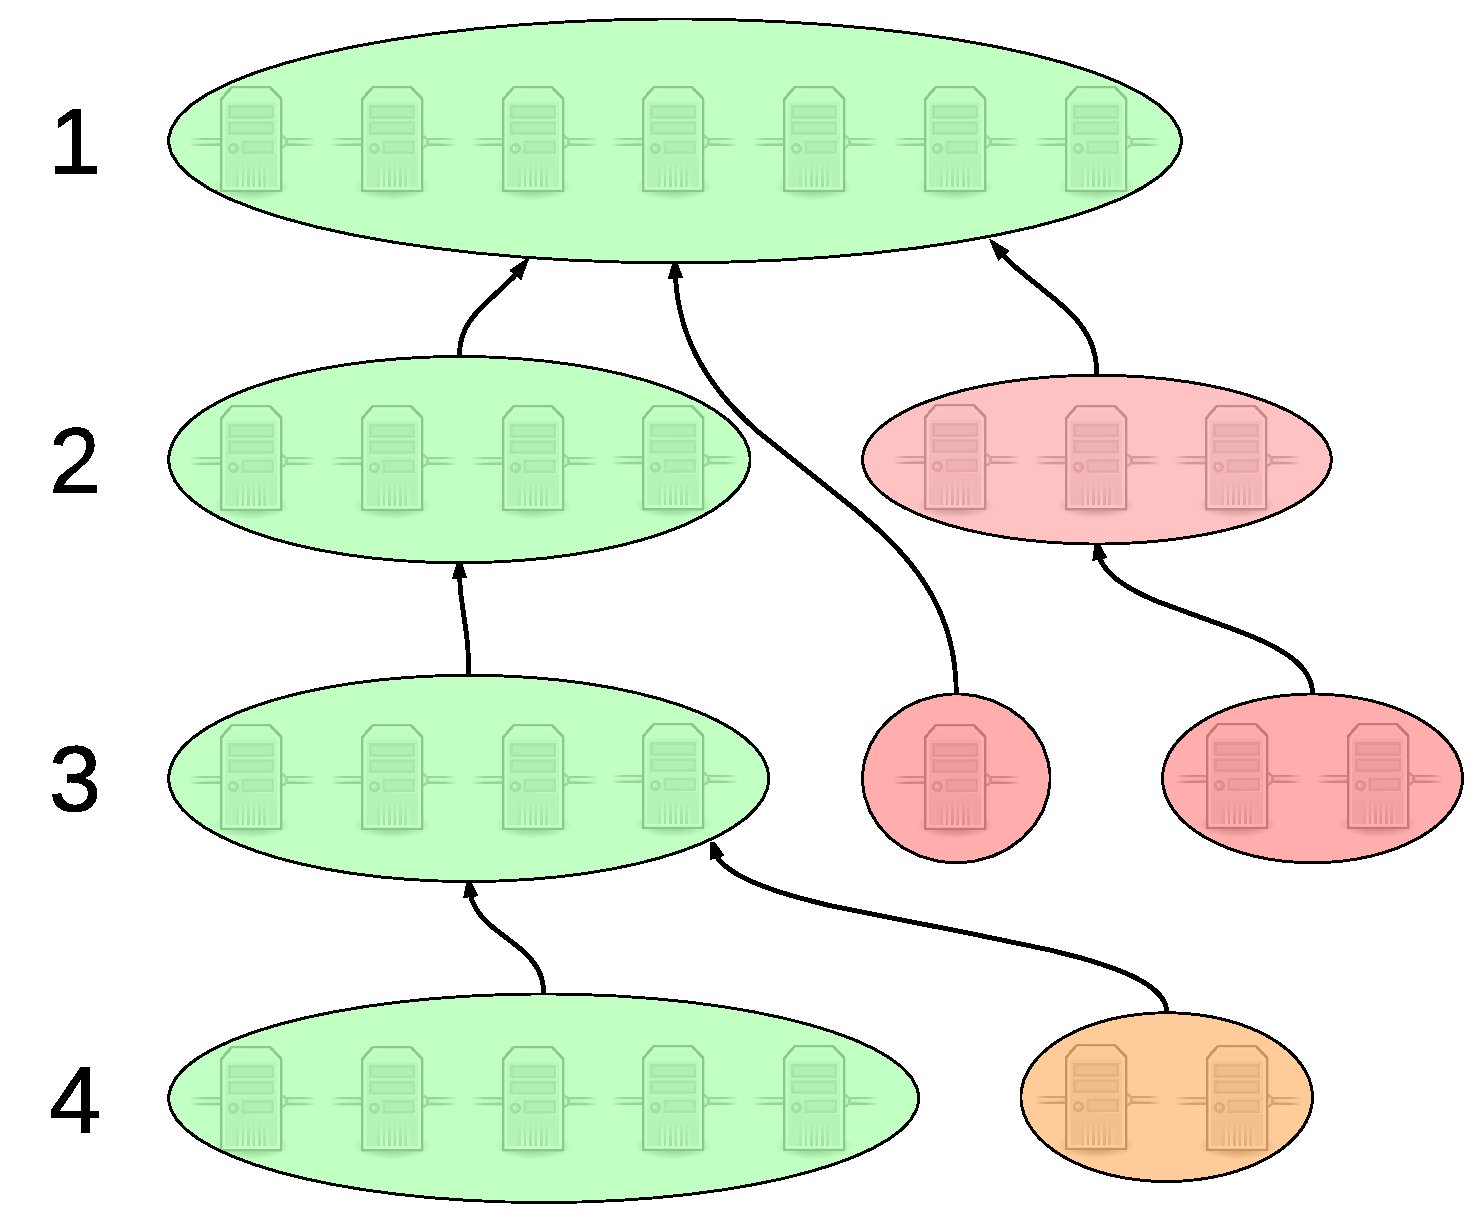
\includegraphics[width=0.65\textwidth]{images/LucidCharts/Page-chain.pdf}
	\caption{An example Pagechain across four Quorums. Each Page contains a references to a previous Page, forming a distributed append-only chain. $ \mathrm{Quorum}_{1} $ is honest and maintains reliable flooding communication, and thus has identical Pages. $ \mathrm{Quorum}_{2} $'s largest cluster is likewise in agreement, but there are three nodes which are acting maliciously together and have changed their Pages. Node 5 in $ \mathrm{Quorum}_{3} $ references an old page in attempt to bypass $ \mathrm{Quorum}_{2} $'s records, and nodes 6-7 are colluding with nodes 5-7 from $ \mathrm{Quorum}_{2} $. Finally, $ \mathrm{Quorum}_{4} $ has two nodes that acted honestly but did not record new records, so their Pagechains differ from the others. However, across all four days the largest clusters are honest nodes and thus integrity remains in the master Pagechain.}
	\label{fig:sidechains}
\end{figure}

\subsection{Client Request}
\label{sec:ClientRequest}

% todo: make diagram of this

Let Bob and Dave be two hidden services, and assume that OnioNS knows a Record from Bob containing an ``example.tor $ \rightarrow $ example0uyw6wgve.onion'' association, and a Record from Dave containing ``example2.tor $ \rightarrow $ example5chqt7to6.onion, sub.example2.tor $ \rightarrow $ example.tor''. Now let Alice request ``sub.example2.tor''.

Since the .tor TLD is not used by the Internet DNS, Alice's client software must direct the request through a Tor circuit to some OnioNS resolver, $ O_{r} $. By default, $ O_{r} $ belongs to the set of Quorum Candidate nodes although Alice may override this and choose some Mirror if she wishes. For security and load reasons, Quorum nodes refuse to respond to queries, so Alice cannot ask them. Following Alice's request, $ O_{r} $ searches its local Pagechain for ``example2.tor'' and finds Dave's Record, which it then sends to Alice. Alice sees the ``sub.example2.tor $ \rightarrow $ example.tor'' association and now queries $ O_{r} $ for ``example.tor''. $ O_{r} $ then locates and sends Bob's Record to Alice. Alice sees that ``example.tor'' has a destination of ``example0uyw6wgve.onion'', and because it has a .onion address she does not need to issue any more queries. Instead, Alice connects to Bob's example0uyw6wgve.onion service via the Tor hidden service protocol and sends her original request (``sub.example2.tor'') to Bob. As is the case with the Internet, Bob's web server may or may not provide specific content to Alice based on this request, but his configuration is outside our scope.

In this way, Alice can query an OnioNS resolver for some Dave-selected domain name and recursively resolve it to a .onion address transparently. The number of resolutions Alice makes is fixed to a maximal length (section \ref{sec:Record}) so this algorithm always completes. We discuss minor optimizations and security enhancements to this procedure in section \ref{sec:ProtoTorClients}.

\section{Primitives}

\subsection{Cryptographic}
\label{sec:CryptoPrim}

OnionNS makes use of cryptographic hash algorithms, digital signatures, proof-of-work, and a pseudorandom number generator.

\begin{itemize}
	\item Let $ H(x) $ be a cryptographic hash function. In our reference implementation we define $ H(x) $ as SHA-384, a truncated and slight modificated derivative of SHA-512. Currently the best preimage attack of SHA-512 breaks 57 out of 80 rounds in $ 2^{511} $ time.\cite{li2012converting} SHA-384 is included in the National Security Agency's Suite B Cryptography for protecting information classified up to Top Secret.
	\item Let $ S_{d}(m, r) $ be a deterministic RSA digital signature function that accepts a message $ m $ and a private RSA key $ r $ and returns an RSA digital signature. Let $ S_{d}(m, r) $ use $ H(x) $ as a digest function on $ m $ in all use cases. In our reference implementation we define $ S_{d}(m, r) $ as EMSA-PSS, (EMSA4) a probabilistic signature scheme defined by PKCS1 v2.1 and republished in 2003's RFC 3447.
	\item Let $ S_{\mathit{ed}}(m, c) $ be an Ed25519 digital signature function that accepts a message $ m $ and a private Curve25519 key $ c $ and returns a 64-byte Ed25519 digital signature. Ed25519 is digital signature scheme designed with high performance, strong implementation security, and minimal keypair and signature sizes objectives in mind. The Ed25519 elliptic curve is birationally equivalent to Curve25519, and Curve25519 keys can be converted to Ed25519 keys in $ \mathcal{O}(1) $ time.\cite{bernstein2011high} Let $ S_{\mathit{ed}}(m, c) $ use $ H(x) $ as a digest function on $ m $ in all use cases.
	\item Let $ V_{\mathit{ed}}(m, C) $ validate an Ed25519 digital signature by accepting a message $ m $ and a public Curve25519 key $ C $, and return true if the signature is valid. Let $ V_{\mathit{ed}}(m, C) $ use $ H(x) $ as a digest function on $ m $ in all use cases.
	\item Let $ \mathrm{PoW}(i) $ be a proof-of-work scheme such as a strong key derivation function that accepts an input key $ k $ and returns a derived key. Our reference implementation uses a fixed salt and scrypt, a password-based key derivation function which is notable for its large memory and CPU requirements during its operation. The scrypt function provides significantly greater resistance to custom hardware attacks and massively parallel computation primarily due to its memory requirements. This limits attackers to the same software implementation and asymptotic cost as legitimate users.\cite{percival2009stronger}\cite{percival2012scrypt} We choose scrypt because of these advantages over other key derivation functions such as SHA-256 or PBKDF2. For these reasons scrypt is also common for proof-of-work purposes in some cryptocurrencies such as Litecoin.
	\item Let $ \mathit{R}(s) $ be a pseudorandom number generator that accepts an initial seed $ s $ and returns a list of numerical pseudorandom numbers. We suggest MT19937, commonly known as the Mersenne Twister. This generator is widely used throughout most programming languages and is well known for its speed, long period, and the high quality of its pseudorandom output, although it is not cryptographically secure.\cite{matsumoto1998mersenne}
\end{itemize}

\subsection{Symbols}

\begin{itemize}
	\item Let $ L_{Q} $ represent size of the Quorum.
	\item Let $ L_{T} $ represent the number of routers in the Tor network.
	\item Let $ L_{P} $ represent the maximum number of Pages in the Pagechain.
	\item Let $ q $ be an Quorum iteration counter.
	\item Let $ \Delta q $ be the lifetime of a Quorum in days: every $ \Delta q $ days $ q $ is incremented by one and a new Quorum is chosen.
	\item Let $ s $ be a Snapshot iteration counter.
	\item Let $ \Delta s $ be the lifetime of a Snapshot in days: every $ \Delta s $ minutes $ s $ is incremented by one, a flood happens, and a fresh Snapshot is used.
\end{itemize}

All textual databases are encoded in JSON. JSON is significantly more compact than XML, but retains readability. Its support of basic primitive types is highly applicable to our needs. Additionally, we consider the JSON format safer than byte-level encoding.

\section{Data Structures}
\label{sec:DataStructures}

\subsection{Record}
\label{sec:Record}

There are five different types of Records: Create, Modify, Move, Renew, and Delete. The latter four Records mimic the format of the Create Record with minor exceptions.

\subsubsection{Create}

A Create record consists of nine components: \emph{type}, \emph{nameList}, \emph{contact}, \emph{timestamp}, \emph{consensusHash}, \emph{nonce}, \emph{pow}, \emph{recordSig}, and \emph{pubHSKey}. Fields that are optional are blank unless specified, and all fields are encoded in base64, except for \emph{nameList} and \emph{timestamp}, which are encoded in standard UTF-8.

\renewcommand{\arraystretch}{1.75} % increase spacing between columns
\begin{center}
    \begin{longtabu}{ | l | c | p{9.5cm} |}
    \hline
    \textbf{Field} & \textbf{Required?} & \textbf{Description} \\
    type & Yes & A textual label containing the type of Record. In this case, \emph{type} is set to ``Create''. \\
    nameList & Yes & An array list of domain names and their destinations. The list of domain names includes one or more second-level domain name, while the remainder of the list contains zero or more subdomains (names at level $ < 2 $) under that second-level domains. In this way, records can be referenced by their unique second-level domain names. Destinations use either .tor or .onion TLDs. \\
    contact & No & Bob's PGP key fingerprint, if he has a key and chooses to disclose it. If the fingerprint is listed, clients may query a public keyserver for this fingerprint, obtain the PGP public key, and contact Bob over encrypted email. \\
    timestamp & Yes & The UNIX timestamp of when the issuer created the registration and began $ \mathrm{PoW}(i) $. \\
    consensusHash & Yes & The hash of the consensus document that generated $ \mathit{Quorum}_{q} $ \\
    nonce & Yes & Four bytes that serve as a source of randomness for $ \mathrm{PoW}(i) $. \\
   	pow & Yes & 16 bytes that store the output of $ \mathrm{PoW}(i) $. \\
   	recordSig & Yes & The output of $ S_{d}(m, r) $ where $ m = \mathit{nameList} \concat \mathit{timestamp} \concat \mathit{consensusHash} \concat \mathit{nonce} \concat \mathit{pow} $ and $ r $ is the hidden service's private RSA key. \\
   	pubHSKey & Yes & Bob's public RSA key. \\
    \hline
    \caption{A Create record, which contains fields common to all records. Every record is self-signed and must have verifiable proof-of-work before it is considered valid.}
    \end{longtabu}
\end{center}

\subsubsection{Modify}

A Modify record allows an owner to update his registration with updated information. The Modify record has identical fields to Create, but \emph{type} is set to ``Modify''. The owner corrects the fields, updates \emph{timestamp} and \emph{consensusHash}, revalidates the proof-of-work, and transmits the record. Modify records have a difficulty of $ \frac{\textrm{difficulty}_{\textrm{Create}}}{4} $. Modify records can be used to add and remove domain names but cannot be used to claim additional second-level domains.

\subsubsection{Move}

% prevents the seller from selling modified records and forcing the buyer to issue a Modify record

A Move record is used to transfer one or more second-level domain names and all associated subdomains from one owner to another. Move records have all the fields of a Create record, have their \emph{type} is set to ``Move'', and contain two additional fields: \emph{target}, a list of domain-destination pairs, and \emph{destPubKey}, the public key of the new owner. Domain names and their destinations contained in \emph{target} cannot be modified; they must match the latest Create, Renew, or Modify record that defined them. Move records also have a difficulty of $ \frac{\textrm{difficulty}_{\textrm{Create}}}{4} $.

\subsubsection{Renew}

% put "page" in italics everywhere?

Second-level domain names (and their associated domain names) expire every $ L $ days because (as explained below) the page-chain has a maximum length of $ L $ pages. Renew records must be reissued periodically at least every $ L $ days to ensure continued ownership of domain names. Renew records are identical to Create records, except that \emph{type} is set to ``Renew''. No modifications to existing domain names can be made in Renew records, and the domain names contained within must already exist in the page-chain. Similar to the Modify and Move records, Renew records have a difficulty of $ \frac{\textrm{difficulty}_{\textrm{Create}}}{4} $.

\subsubsection{Delete}

% attacker could compromise key, issues Move record before original owner knew of compromise. Or attacker could then reclaim domain name

If a owner's private key is compromised or if they wish to relinquish ownership rights over all of their domain names, they can issue a Delete record. Aside from their \emph{type} field set to ``Delete'', Delete records are identical in form to Create records but have the opposite effect: all second-level domains contained within the record are purged from local caches and made available for others to claim. There is no difficulty associated with Delete records, so they can be issued instantly.

\subsection{Snapshot}

Snapshots contain four fields: \emph{originTime}, \emph{recentRecords}, \emph{fingerprint}, and \emph{snapshotSig}.

\begin{description}
	\item[originTime] \hfill \\
		Unix time when the snapshot was first created.
	\item[recentRecords] \hfill \\
		A array list of records in reverse chronological order by receive time.
	\item[fingerprint] \hfill \\
		The hash of the public key of the machine maintaining this snapshot. This is the Tor fingerprint, a unique identification string widely used throughout Tor infrastructure and third-party tools to refer to specific Tor nodes.
	\item[snapshotSig] \hfill \\
		The output of $ S_{\mathit{ed}}(\mathit{originTime} \concat \mathit{recentRecords} \concat \mathit{fingerprint}], c) $ where $ c $ is the machine's private Curve25519 NTor key.
\end{description}

\subsection{Page}

Each page contains five fields, \emph{prevHash}, \emph{recordList}, \emph{consensusDocHash}, \emph{fingerprint}, and \emph{pageSig}.

\begin{description}
	\item[prevHash] \hfill \\
		The SHA-384 hash of \emph{prevHash}, \emph{recordList}, and \emph{consensusDocHash} of a previous page.
	\item[recordList] \hfill \\
		An array list of records, sorted in a deterministic manner.
	\item[consensusDocHash] \hfill \\
		The SHA-384 of $ cd $.
	\item[fingerprint] \hfill \\
		The hash of the public key of the machine maintaining this page, the Tor fingerprint.
	\item[pageSig] \hfill \\
		The output of $ S_{\mathit{ed}}(H(\mathit{prevHash} \concat \mathit{recordList} \concat \mathit{consensusDocHash})], c) $ where $ c $ is the machine's private Curve25519 NTor key.
\end{description}

\section{Protocols}
\label{sec:Protocols}

Throughout this section, when a party downloads consensus documents, they can safely obtain them from any source because they can validate the signatures on the documents against the Tor authority public keys to ensure that they were not modified in transit. Several online sources archive consensus documents and make them available retrospectively; in our reference implementation we also introduce another source. Note that in practice it is often more efficient to download consensus documents en-masse as they achieve very high compression ratios under 7zip.

% todo: the examples here aren't valid

\subsection{Hidden Services}
\label{sec:ProtoHiddenServices}

\subsubsection{Record Generation}

Mirrors and Tor clients check the validity of Records that they receive through synchronization or query responses, respectively. Invalid Records will be rejected by all parties, so Bob must generate a valid Record before broadcast.

\begin{enumerate}
	\item Bob selects the value for \emph{type} based on the desired operation.
	\item Bob constructs the \emph{nameList} domain-destination associations.
	\item Bob provides his PGP key fingerprint in \emph{contact} or leaves it blank if he doesn't have a PGP key or if he chooses not to disclose it. Bob can derive his PGP fingerprint with the ``gpg --fingerprint'' Unix command.
	\item Bob records the number of seconds since the Unix epoch in \emph{timestamp}.
	\item Bob sets \emph{consensusHash} to the output of $ H(x) $, where $ x $ is the consensus document published at 00:00 GMT on day $ \floor[\big]{\frac{q}{\Delta q}} $.
	\item Bob initially defines \emph{nonce} as four zeros.
	\item Let $ \mathit{central} $ be $\mathit{type} \concat \mathit{nameList} \concat \mathit{contact} \concat \mathit{timestamp} \concat \mathit{consensusHash} \concat \mathit{nonce} $.
	\item Bob sets \emph{pow} as $ \mathrm{PoW}(\mathit{central}) $.
	\item Bob sets \emph{recordSig} as the output of $ S_{d}(m, r) $ where $ m = \mathit{central} \concat \mathit{pow} $ and $ r $ is Bob's private RSA key.
	\item Bob saves the PKCS.1 DER encoding of his RSA public key in \emph{pubHSKey}.
\end{enumerate}

Bob then must increment \emph{nonce} and reset \emph{pow} and \emph{recordSig} until $ H(\mathit{central} \concat \mathit{pow} \concat \mathit{recordSig}) \leq 2^{\mathit{difficulty} * \mathit{count}} $ where \emph{difficulty} is a fixed constant that specifies the work difficulty and \emph{count} is the number of second-level domain names claimed in the Record. An example of a completed and valid record is shown in Figure \ref{fig:sampleRecord}.

\begin{figure}
	\begin{lstlisting}
	{
		"names": {
			"example.tor": "exampleruyw6wgve.onion"
		}
		"contact": "AD97364FC20BEC80",
		"timestamp": 1424045024,
		"consensusHash": "uU0nuZNNPgilLlLX2n2r+sSE7+N6U4DukIj3rOLvzek=",
		"nonce": "AAAABw==",
		"pow": "4I4dzaBwi4AIZW8s2m0hQQ==",
		"recordSig": 	"KSaOfzrXIZclHFcYxI+3jBwLs943wxVv3npI5ccY/kBEpyXRSopzjoFs746n0tJqUpdY4Kbe6DBwERaN7ELmSSK9Pu6q8QeKzNAh+QOnKl0fKBN7fqowjkQ3ktFkR0Vuox9WrrbNTMa4+up0Np52hlbKA3zSRz4fbR9NVlh6uuQ=",
		"pubHSKey": "MIGhMA0GCSqGSIb3DQEBAQUAA4GPADCBiwKBgQDE7CP/kgwtJhTTc4JpuPkvA7Ln9wgc+fgTKgkyUp1zusxgUAn1c1MGx4YhO42KPB7dyZOf3pcRk94XsYFY1ULkF2+tf9KdNe7GFzJyMFCQENnUcVXbcwLH4vAeiGK7R/nScbCbyc9LT+VE1fbKchTL1QzLVBLqJTxhR+9YPi8x+QIFAdZ8BJs="
	}
	\end{lstlisting}
	\caption{A sample registration record. The textual fields are in UTF-8, while the binary fields are in base64. The structure is encoded in JSON.}
	\label{fig:sampleRecord}
\end{figure}

\subsubsection{Record Validation}

% todo: Q member must check that the HS exists, and that no more than 2 domains go to that key

Let Carol be a Tor client or a Mirror that receives a Record from another Mirror. Bob must also perform these procedures to ensure that he sends a valid Record.

\begin{enumerate}
	\item Carol checks that the Record contains valid JSON.
	\item Carol checks that \emph{type} is either ``Create'', ``Modify'', ``Move'', ``Renew'', or ``Delete''.
	\item Carol checks that \emph{nameList} is has a length $ \in [1,24] $, contains at least one second-level domain name, and that all subdomains have a second-level domain name within \emph{nameList}. Additionally, Carol checks that there is no domain name nor destination that uses more than 16 names, that is longer than 32 characters, or whose total length is more than 128 characters.
	\item Carol checks that \emph{contact} is either 0, 16, 24, or 32 characters in length, and that \emph{contact} is valid hexadecimal.
	\item Carol checks that \emph{timestamp} is not in the future nor more than 48 hours old relative to her system clock.
	\item Carol checks that \emph{pubHSKey} is a valid PKCS.1 DER-encoded public 1024-bit RSA key, and that when converted to a .onion address that address appears at least once in \emph{nameList}.
	\item Carol checks the validity of \emph{recordSig} deterministic signature against \emph{pubHSKey} and $ \mathit{central} \concat \mathit{pow} $.
	\item Carol obtains the $ \floor[\big]{\frac{q}{\Delta q}} $ 00:00 GMT consensus document and checks $ H(x) $ on it against \emph{consensusHash}. She also confirms that the consensus document is no older than $ \mathrm{min}(48, 12 * \Delta q) $.
	\item Carol checks that $ H(\mathit{central} \concat \mathit{pow} \concat \mathit{recordSig}) \leq 2^{\mathit{difficulty} * \mathit{count}} $
	\item Carol calculates $ \mathrm{pow}(\mathit{central}) $ and confirms that the output matches \emph{nonce}.
\end{enumerate}

If at any step an assertion fails, the Record is not valid and Carol does not accept it.

\subsubsection{Record Broadcast}

% Page Selection protocol may be useful here

\begin{enumerate}
	\item Bob derives the current Quorum by the Quorum Derivation protocol described in section \ref{sec:ProtoTorClients}.
	\item Bob constructs a circuit, $ c_{1} $, to a Mirror node $ m_{1} $.
	\item Bob asks for and receives from $ c_{1} $ the $ H(\mathit{prevHash} \concat \mathit{recordList} \concat \mathit{consensusDocHash}) $ hash and \emph{pageSig} (the ed25519 signature on that hash) from each Quorum node.
	\item Bob confirms via $ V_{\mathit{ed}}(m, C) $ each \emph{pageSig} and defines $ U $ as the largest set of Quorum nodes that have the same hash. % todo: this cluster could be malicious, this isn't guarenteed safe.
	\item Bob randomly chooses a node $ n_{1} $ from $ U $ and builds a circuit to it, $ c_{2} $.
	\item Bob uploads his Record through $ c_{2} $ to $ n_{1} $.
	\item Bob waits up to $ \Delta s $ minutes for the next $ s $ flood iteration.
	\item Bob uses $ c_{1} $ to ask $ m_{1} $ for any second-level domain name contained in his Record.
	\item Bob has confirmation that his Record was accepted and processed by the Quorum if $ m_{1} $ returns the Record he uploaded, assuming $ m_{1} $ is not malicious and is synchronizing against a node other than $ n_{1} $.
	\item If $ m_{1} $ does not return Bob's Record, he can either query another Mirror or repeat this procedure and broadcast to a different Quorum node. This choice is left up to the operator.
\end{enumerate}

%For security purposes, the operator should use the same entry node for this transmission that their hidden service uses for its communication. todo: need cite

\subsection{OnioNS Servers}
\label{sec:ProtoOnioNServers}

Let Charlie be the name of an OnioNS Mirror.

\subsubsection{Database Initialization}

\begin{enumerate}
	\item Charlie creates a empty Snapshot.
	\item Charlie sets \emph{originTime} to the number of seconds since the Unix epoch.
	\item Charlie sets \emph{recentRecords} to an empty array.
	\item Charlie sets \emph{fingerprint} to his Tor fingerprint.
	\item Charlie sets $ \mathit{snapshotSig} = S_{\mathit{ed}}(\mathit{originTime} \concat \mathit{recentRecords} \concat \mathit{fingerprint}, c) $ where $ c $ is Charlie's private Curve25519 NTor key.
	\item Charlie begins listening for incoming Records.
	\item Charlie creates an initial Page $ P_{\mathit{curr}} $.
	\item Charlie selects a previous Page $ P_{\mathit{prev}} $ to back-reference via the Page Selection protocol.
	\item Charlie sets $ \mathit{prevHash} = H(P_{\mathit{prev}}(\mathit{prevHash} \concat \mathit{recordList} \concat \mathit{consensusDocHash}) $.
	\item Charlie sets \emph{recordList} to an empty array.
	\item Charlie downloads from some remote source the consensus document $ \mathit{cd} $ issued on day $ \floor[\big]{\frac{q}{\Delta q}} $ at 00:00 GMT and authenticates it against the Tor authority public keys.
	\item Charlie sets $ \mathit{consensusDocHash} = H(\mathit{cd}) $.
	\item Charlie sets \emph{fingerprint} to his Tor fingerprint.
	\item Charlie sets $ \mathit{pageSig} = S_{\mathit{ed}}(H(\mathit{prevHash} \concat \mathit{recordList} \concat \mathit{consensusDocHash}), c) $ where $ c $ is Charlie's private Curve25519 NTor key.
\end{enumerate}

\begin{figure}
	\begin{lstlisting}
	{
		"prevHash": 0,
		"recordList": [],
		"consensusDocHash": "uU0nuZNNPgilLlLX2n2r+sSE7+N6U4DukIj3rOLvzek=",
		"fingerprint": "2FC06226AE152FBAB7620BB107CDEF0E70876A7B",
		"pageSig": "KSaOfzrXIZclHFcYxI+3jBwLs943wxVv3npI5ccY/kBEpyXRSopzjoFs746n0tJqUpdY4Kbe6DBwERaN7ELmSSK9Pu6q8QeKzNAh+QOnKl0fKBN7fqowjkQ3ktFkR0Vuox9WrrbNTMa4+up0Np52hlbKA3zSRz4fbR9NVlh6uuQ="
	}
	\end{lstlisting}
	\caption{A sample empty Page.}
	\label{fig:emptyPage}
\end{figure}

\begin{figure}
	\begin{lstlisting}
	{
		"originTime": 1426507551,
		"recentRecords": [],
		"fingerprint": "2FC06226AE152FBAB7620BB107CDEF0E70876A7B",
		"snapshotSig": "KSaOfzrXIZclHFcYxI+3jBwLs943wxVv3npI5ccY/kBEpyXRSopzjoFs746n0tJqUpdY4Kbe6DBwERaN7ELmSSK9Pu6q8QeKzNAh+QOnKl0fKBN7fqowjkQ3ktFkR0Vuox9WrrbNTMa4+up0Np52hlbKA3zSRz4fbR9NVlh6uuQ="
	}
	\end{lstlisting}
	\caption{A sample empty Snapshot.}
	\label{fig:emptySnapshot}
\end{figure}

\subsubsection{Page Selection}

The Page Selection protocol is used to select a Page in the midst of Page disagreements between current or past Quorum members. It relies on our original design assumption that the largest set of Quorum nodes with agreeing and valid Pages are acting honestly, so by extension the Page they maintain is honest as well and we can safely choose it. Let $ P_{c} $ be the Page that Charlie has selected.

% what happens if pageSig doesn't validate?

\begin{enumerate}
	\item Charlie obtains the set of Pages maintained by $ \mathit{Quorum}_{q} $.
	\item Charlie obtains the consensus document $ \mathit{cd} $ issued on day $ \floor[\big]{\frac{q}{\Delta q}} $ at 00:00 GMT and authenticates it against the Tor authority public keys.
	\item Charlie uses $ \mathit{cd} $ to calculate the Quorum via the Quorum Derivation protocol.
	\item For each Page,
		\begin{enumerate}
			\item Charlie checks that \emph{prevHash} references some page from the previous Quorum.
			\item Charlie calculates $ h = H(\mathit{prevHash} \concat \mathit{recordList} \concat \mathit{consensusDocHash}) $.
			\item Charlie checks that $ \mathit{fingerprint} $ is a member of $ \mathit{Quorum}_{q} $.
			\item Charlie checks that $ V_{\mathit{ed}}(h, C) $ returns true where $ C $ is $ \mathit{fingerprint} $'s public Curve25519 key.
		\end{enumerate}
	\item Charlie sorts the set of Pages by $ h $, and constructs a 2D array of Pages that have the same $ h $.
	\item For each set of Pages with equal $ h $,
		\begin{enumerate}
			\item Charlie checks that $ \mathit{consensusDocHash} = H(\mathit{cd}) $.
			\item Charlie checks each Record in \emph{recordList} via the Record Validation protocol.
		\end{enumerate}
	\item If the validation of a Page fails, Charlie removes it from the equal-$ h $ list.
	\item Let $ P_{c} $ be chosen arbitrarily from the largest set of valid Pages with equal $ h $.
\end{enumerate}

In this way, Charlie need not preform a deep verification of all Pages from $ \mathit{Quorum}_{q} $ in order to choose a Page.

\subsubsection{Pagechain Validation}

% available i means max(0, L_{P})

Assume that Charlie has obtained a complete Pagechain. Let $ P_{c} $ be an initial empty Page and let $ f(P_{1}, P_{2}, q) $ accept two Pages and return true if $ P_{1} = P_{2} $ or if $ q = 0 $. For each $ q $ from the oldest available $ q $ to the most recent $ q $,

\begin{enumerate}
	\item Charlie chooses a Page $ P_{c2} $ from $ \mathit{Quorum}_{q} $ via the Page Selection Protocol.
	\item Charlie checks that $ f(P_{c}, P_{c2}, q) $ returns true, or repeats step 1 to choose another Page from the next largest set of Pages that have equal $ h $.
\end{enumerate}

\subsubsection{Synchronization}

\begin{enumerate}
	\item Charlie randomly selects a Quorum Candidate, $ R_{j} $.
	\item Charlie downloads $ R_{j} $'s Pagechain and the Pages used by each Quorum member for each Quorum, obtaining a 2D data structure at most $ L_{P} $ Pages long and $ L_{Q} $ Pages wide.
	\item Charlie checks the downloaded Pagechain via the Pagechain Validation protocol. If it does not validate, Charlie picks another Quorum Candidate $ R_{k} $, $ k /ne j $, and downloads the invalid Pages from $ R_{k} $.
	\item Charlie randomly selects a Quorum node $ Q_{c} $.
	\item Charlie periodically polls $ Q_{c} $ for the Pages of all other Quorum nodes.
	\item When a set of Pages is available from $ Q_{c} $, Charlie follows the Page Selection protocol to choose a Page that becomes the new Pagechain head.
\end{enumerate}

\subsubsection{Quorum Qualification}

The Quorum is the OnioNS most trusted set of authoritative nodes. They have responsibility over the master Pagechain, are responsible for handling incoming Records from hidden service operators, and Mirrors poll them for their most recent Page. As such, the Quorum must be derived from the most reliable, capable, and trusted Tor nodes and more importantly Quorum nodes must be up-to-date Mirrors. These two requirements are crucial to ensuring the reliability and security of the Quorum.

The first criteria requires Tor nodes to demonstrate that they sufficient capabilities to handle the increase in communication and processing from with OnioNS protocols. Fortunately, Tor's infrastructure already provides a mechanism that can be utilized to demonstrate this requirement; Tor authority nodes assign flags to Tor routers to classify their capabilities, speed, or uptime history: these flags are used for circuit generation and hidden service infrastructure. Let Tor nodes meet the first qualification requirement if they have the Fast, Stable, Running, and Valid flags. As of February 2015, out of the $ \approx $ 7,000 nodes participating in the Tor network, $ \approx $ 5,400 of these node have these flags and complete the second requirement.\cite{TorMetrics}

To demonstrate the second criteria, the na\"{i}ve solution is to simply ask nodes meeting the first criteria for their Page, and then compare the recency of its latest Page against the Pages from the other nodes. However, this solution does not scale well; Tor has $ \approx $ 2.25 million daily users\cite{TorMetrics}: it is infeasible for any single node to handle queries from all of them. Instead, let each Mirror that meets the first criteria perform the following:

\begin{enumerate}
	\item Charlie calculates $ t = H(\mathit{pc} \concat \floor[\big]{\frac{m - 15}{30}}) $ where \emph{pc} is Charlie's Pagechain and $ m $ is the minute component of the time of day in GMT. Tor's consensus documents are published at the top of each hour; we manipulate $ m $ such that $ t $ is consistent at the top of each hour even with at most a 15-minute clock-skew.
	\item Let Charlie convert $ t $ to base64 and truncate to 8 bytes.
	\item Let Charlie include this new $ t $ in the Contact field in his relay descriptor sent to Tor authority nodes.
\end{enumerate}

While ideally $ t $ could be placed inside a new field within the relay descriptor, to ease integration with existing Tor infrastructure and third-party tools we use the Contact field, a user-defined optional entry that Tor relay operators typically use to list methods of contact such as an email address. OnionNS would not be the first system to embed special information in the Contact field: PGP keys and BTC addresses commonly appear in the field, especially for high-performance routers.

\subsubsection{Record Processing}

A Quorum node $ Q_{j} $ listens for new Records from hidden service operators. When a Record is received, $ Q_{j} $

\begin{enumerate}
	\item $ Q_{j} $ rejects the Record if it does not validate according to the Record Validation protocol.
	\item If it is a Create record, $ Q_{j} $ rejects it if any of its second-level domains already exist in $ Q_{j} $'s Pagechain.
	\item If it is a Modify, Move, Renew or Delete Record, $ Q_{j} $ rejects it if either of the following are true:
		\begin{enumerate}
			\item It was not found in the Pagechain.
			\item Its \emph{pubHSKey} does not match the latest Record found in the Pagechain under its second-level domain names.
		\end{enumerate}
	\item If $ Q_{j} $ has rejected the Record, $ Q_{j} $ informs Bob of this outcome and its reason.
	\item If $ Q_{j} $ has not rejected the Record,
		\begin{enumerate}
			\item $ Q_{j} $ informs Bob that his Record was accepted.
			\item $ Q_{j} $ merges the Record into its current Snapshot as shown in Figure \ref{fig:recordInSS}.
			\item $ Q_{j} $ regenerates \emph{snapshotSig}.
		\end{enumerate}
\end{enumerate}

\begin{figure}
	\begin{lstlisting}
	{
		"originTime": 1426507551,
		"recentRecords": [{
			"names": {
				"example.tor": "exampleruyw6wgve.onion"
			}
			"contact": "AD97364FC20BEC80",
			"timestamp": 1424045024,
			"consensusHash": "uU0nuZNNPgilLlLX2n2r+sSE7+N6U4DukIj3rOLvzek=",
			"nonce": "AAAABw==",
			"pow": "4I4dzaBwi4AIZW8s2m0hQQ==",
			"recordSig": 	"KSaOfzrXIZclHFcYxI+3jBwLs943wxVv3npI5ccY/kBEpyXRSopzjoFs746n0tJqUpdY4Kbe6DBwERaN7ELmSSK9Pu6q8QeKzNAh+QOnKl0fKBN7fqowjkQ3ktFkR0Vuox9WrrbNTMa4+up0Np52hlbKA3zSRz4fbR9NVlh6uuQ=",
			"pubHSKey": "MIGhMA0GCSqGSIb3DQEBAQUAA4GPADCBiwKBgQDE7CP/kgwtJhTTc4JpuPkvA7Ln9wgc+fgTKgkyUp1zusxgUAn1c1MGx4YhO42KPB7dyZOf3pcRk94XsYFY1ULkF2+tf9KdNe7GFzJyMFCQENnUcVXbcwLH4vAeiGK7R/nScbCbyc9LT+VE1fbKchTL1QzLVBLqJTxhR+9YPi8x+QIFAdZ8BJs="
		}],
		"fingerprint": "2FC06226AE152FBAB7620BB107CDEF0E70876A7B",
		"snapshotSig": "KSaOfzrXIZclHFcYxI+3jBwLs943wxVv3npI5ccY/kBEpyXRSopzjoFs746n0tJqUpdY4Kbe6DBwERaN7ELmSSK9Pu6q8QeKzNAh+QOnKl0fKBN7fqowjkQ3ktFkR0Vuox9WrrbNTMa4+up0Np52hlbKA3zSRz4fbR9NVlh6uuQ="
	}
	\end{lstlisting}
	\caption{A sample Create Record has been merged into an initially-blank Snapshot.}
	\label{fig:recordInSS}
\end{figure}

\subsubsection{Flooding}

% an adversary could cause a denial of service by creating a Page with many false PoWs, causing Quorum nodes to perform a lot of PoW checks

% todo: search for "Delta i"

% pass H(page, fingerprint) to each other before exchanging page signatures? This slows collusion. Ask for this hash. analysis on this

% domain expiration if server unavailable, expiration of domain names by quorums, two quorums must agree, grace period

%Once received, Carol validates the record by checking the fields, the signature, and the proof-of-work. Carol accept the record if it passes. Carol has no previous knowledge of ``example.tor'' so there are no conflicts. Carol then adds the Create record into her current snapshot as shown in Figure \ref{fig:recordInSS}.

Every $ \Delta s $ minutes, a burst of communication happens between Quorum nodes wherein Snapshots and Page signatures are flooded between them. This allows Quorum nodes to hear new Records and to know the status of the Pages maintained by their brethren. The exact timing of this protocol is dependent on the local system clock of each Quorum node. Let $ Q_{j} $ be a Quorum node with current Snapshot $ s_{s} $, and at the $ \Delta s $ mark,

\begin{enumerate}
	\item $ Q_{j} $ generates a new Snapshot, $ s_{s+1} $ via the Database Initialization protocol.
	\item $ Q_{j} $ sets $ s_{s+1} $ to be the current Snapshot, used to collect new Records.
	\item $ Q_{j} $ sets $ p_{\mathit{old}} $ to the current Page.
	\item For every $ Q_{k} $ Quorum node, $ k \ne j $,
		\begin{enumerate}
			\item $ Q_{j} $ asks $ Q_{k} $ for his snapshot.
			\item $ Q_{j} $ merges the Records within $ Q_{k} $'s \emph{recentRecords} into $ Q_{j} $'s current Page, as shown in Figure \ref{fig:pageMerge}.
			\item $ Q_{j} $ asks $ Q_{k} $ for its Page and sets the response as $ s_{k} $.
			\item $ Q_{j} $ calculates $ s_{k} $'s $ h $ value (see the Page Selection protocol) and if it matches a Page $ g $ already known to $ Q_{j} $, $ Q_{j} $ archives an association between $ Q_{k} $ and $ g $. In this case $ s_{k} $'s \emph{pageSig} will validate $ g $'s $ h $, allowing the width of the Pagechain to be grouped efficiently. Otherwise, $ Q_{j} $ archives $ s_{k} $.
		\end{enumerate}
	\item $ Q_{j} $ regenerates \emph{pageSig}.
	\item $ Q_{j} $ sends $ s_{s} $ when another Quorum node requests his Snapshot.
	\item $ Q_{j} $ sends $ p_{\mathit{old}} $ when a Mirror or a Quorum node asks for his Page.
\end{enumerate}

\begin{figure}
	\begin{lstlisting}
	{
		"prevHash": "4I4dzaBwi4AIZW8s2m0hQQ==",
		"recordList": [{
			"names": {
				"example.tor": "exampleruyw6wgve.onion"
			}
			"contact": "AD97364FC20BEC80",
			"timestamp": 1424045024,
			"consensusHash": "uU0nuZNNPgilLlLX2n2r+sSE7+N6U4DukIj3rOLvzek=",
			"nonce": "AAAABw==",
			"pow": "4I4dzaBwi4AIZW8s2m0hQQ==",
			"recordSig": 	"KSaOfzrXIZclHFcYxI+3jBwLs943wxVv3npI5ccY/kBEpyXRSopzjoFs746n0tJqUpdY4Kbe6DBwERaN7ELmSSK9Pu6q8QeKzNAh+QOnKl0fKBN7fqowjkQ3ktFkR0Vuox9WrrbNTMa4+up0Np52hlbKA3zSRz4fbR9NVlh6uuQ=",
			"pubHSKey": "MIGhMA0GCSqGSIb3DQEBAQUAA4GPADCBiwKBgQDE7CP/kgwtJhTTc4JpuPkvA7Ln9wgc+fgTKgkyUp1zusxgUAn1c1MGx4YhO42KPB7dyZOf3pcRk94XsYFY1ULkF2+tf9KdNe7GFzJyMFCQENnUcVXbcwLH4vAeiGK7R/nScbCbyc9LT+VE1fbKchTL1QzLVBLqJTxhR+9YPi8x+QIFAdZ8BJs="
		}],
		"consensusDocHash": "uU0nuZNNPgilLlLX2n2r+sSE7+N6U4DukIj3rOLvzek=",
		"fingerprint": "2FC06226AE152FBAB7620BB107CDEF0E70876A7B",
		"pageSig": "KSaOfzrXIZclHFcYxI+3jBwLs943wxVv3npI5ccY/kBEpyXRSopzjoFs746n0tJqUpdY4Kbe6DBwERaN7ELmSSK9Pu6q8QeKzNAh+QOnKl0fKBN7fqowjkQ3ktFkR0Vuox9WrrbNTMa4+up0Np52hlbKA3zSRz4fbR9NVlh6uuQ="
	}
	\end{lstlisting}
	\caption{A Page containing an example Record. This Page is the result of the Snapshot in Figure \ref{fig:recordInSS} into an empty Page.}
	\label{fig:pageMerge}
\end{figure}

\subsection{Tor Clients}
\label{sec:ProtoTorClients}

Let Alice be a Tor client. We assume now that Alice has chosen Charlie as her domain resolver and that Charlie is not a member of the current Quorum.

\subsubsection{Quorum Derivation}

\begin{enumerate}
	\item Alice obtains a copy of the most recent consensus document, $ cd $, published on day $ \floor[\big]{\frac{q}{\Delta q}} $ at 00:00 GMT.
	\item Alice scans $ cd $ and constructs a list \emph{qc} of Quorum Candidates of Tor routers that have the Fast, Stable, Running, and Valid flags and that are in the largest set of Tor routers that publish an identical time-based hash, as described in the Quorum Qualification protocol. She can construct \emph{qc} in $ \mathcal{O}(L_{T}) $ time.
	\item Alice constructs $ f = \mathit{R}(H(\mathit{cd}) $.
	\item Alice uses \emph{f} to randomly scramble \emph{qc}.
	\item The first $ \mathrm{min}(\mathrm{size}(\mathit{qc}), L_{Q}) $ routers are the Quorum.
\end{enumerate}

\subsubsection{Domain Query}

There are three verification levels in a Domain Query, each providing progressively more verification to Alice that the Record she receives is authentic, unique, and trustworthy. At verification 0, the default:

% use case diagram of this?

\begin{enumerate}
	\item Alice constructs a Tor circuit to Charlie, so from Charlie's perspective she is anonymous.
	\item Alice provides a .tor domain name $ d $ into the Tor Browser. The Internet has no .tor TLD, so $ d $ is not processed as a traditional domain name would be.
	\item \label{step:trim} If $ d $'s highest-level name is ``www'', Alice removes that name.
	\item \label{step:level} Alice asks Charlie for the most recent Record $ r $ associated with $ d $ at verification level 0.
	\item Charlie reviews his Pagechain reverse-chronological order until he finds a Record containing $ d $, which he returns to Alice.
	\item Alice validates $ r $ via the Record Validation protocol. If it does not validate, she changes to another resolver and repeats this protocol.
	\item If the destination for $ d $ in $ r $ uses a .tor TLD, $ d $ becomes that destination and Alice jumps back to step \ref{step:trim}.
	\item Otherwise, the destination must have a .onion TLD, which Alice looks up by the Tor hidden service protocol.
	\item Alice checks that $ r $'s \emph{pubHSKey} matches the one in Tor's distributed hash table.
	\item Alice sends the original $ d $ to the hidden service.
\end{enumerate}

Verification level 1 proceeds nearly identical to level 0. Alice sends ``level 1'' to Charlie in step \ref{step:level} and Charlie returns the Page $ p $ containing $ r $. Then Alice can check the integrity of $ p $ via the Page Selection protocol and can verify its authenticity via checking that $ V_{\mathit{ed}}(m, C) $ returns true when $ m $ is the Page hash $ h $ and $ C $ is \emph{fingerprint}'s public Curve25519 NTor key.

At Verification level 2, Alice sends ``level 2'' to Charlie in step \ref{step:level} and Charlie returns $ p $ from level 1 and all digital signatures on $ h $ from all Quorum nodes that agreed on $ p $. Then Alice can perform width verification: she can see that a large percentage of Quorum nodes maintained $ p $, thus increasing the trustworthiness of both $ p $ and $ r $.

Alice can be certain that the Record $ r $ she receives is authentic and that it contains a domain name $ d $ that is unique by performing a full Synchronization and obtaining Charlie's Pagechain for herself, but this is impractical in most environments. It cannot be safely assumed that Alice has storage capacity to hold all the Pages in the Pagechain. Additionally, Tor's median circuit speed is often less than 1 MiB/s,\cite{TorMetrics} so for convenience data transfer must be minimized. Therefore Alice can simply fetch minimal information and rely on her trust of Charlie and the Quorum.

\subsubsection{Onion Query}

Alice may also issue a reverse-hostname lookup to Charlie to find second-level domains that resolve to a given .onion address. This request is known as an Onion Query. Charlie performs a reverse-chronological search in the Pagechain for Records that .onion as a destination and returns the results corresponding to the verification level. Onion Queries have a high likelihood of failure as not every .onion name has a corresponding .tor domain name, but all OnioNS domain names will have Forward-Confirmed Reverse DNS match.

\section{Optimizations}

There are several improvements that be made upon the basic design protocols that significantly enhance the performance of Mirrors when responding to Domain or Onion Requests. We also introduce the Hashtable Bitset data structure, which improves security on the client end.

\subsection{AVL Tree}

An AVL tree is a self-balancing binary search tree with $ \mathcal{O}(\mathrm{log}(n)) $ time for search, insert, and delete. OnioNS mirrors can cache all the Records in its local Pagechain in an AVL tree. After the Pagechain is validated, the Mirror iterates through the Pagechain in chronological order and constructs a list of associations between a second-level domain name and the location in the Pagechain of the Record containing that domain. The Mirror then inserts that list into the AVL tree, where sorting occurs by alphabetical comparison of domain names. This effectively transforms the lookup time of Records for Domain Queries from $ \mathcal{O}(n) $ to $ \mathcal{O}(\mathrm{log}(n)) $ in the worst case.

As the Mirror handles new Records sent to Quorum nodes, it must update this AVL tree. Create Records trigger an insert operation, Delete Records cause a deletion, and all other Records update a location pointer to the more recent Record.

% todo: illustration of an AVL tree with pointers to page-chain records

\subsection{Trie}

We also suggest utilizing a trie, a digital tree, for efficiently structuring .onion addresses and optimizing Onion Query lookups. If each node in the trie is a character in the .onion address, the trie has a branching factor of 58 and a maximum depth of 16. Let the leaves of the trie be the location of the most recent Record in the Pagechain that has that address as a destination. Like the AVL tree, Mirrors must take care to update the trie cache when processing new Records, but this is efficient as trie search, insertion, and deletion all occur in $ \mathcal{O}(1) $.

\subsection{Hashtable Bitset}
\label{sec:HashtableBitset}

A hashtable bitset is a special and highly compact adaptation of a traditional hashtable. We introduce a hashtable bitset for two purposes: 1) to prove the non-existence of a domain name, and 2) to improve the efficiency of lookups for non-existent domain names from $ \mathcal{O}(\mathrm{log}(n)) $ through the AVL tree to $ \mathcal{O}(1) $ time. This first property is a challenge often overlooked in other domain name systems: even if domain names can be authenticated by a client (e.g. OnioNS Records or SSL certificates) a DNS resolver may lie about the non-existence and claim a false negative. In OnioNS, Alice can download the entire Pagechain and confirm for herself, but as we stated earlier this is not practical. Alice could also query another trusted source such as Quorum Candidates, but this approach does not scale well. Instead, a trusted authority can sign a hashtable bitset once and allow Mirrors to prove non-existence for any domain name.

As an extension of an ordinary hashtable, the hashtable bitset maps keys to buckets, but here we only track the existence of a key but not the keys themselves. Therefore each bucket in the structure is represented as a bit, creating a compact $ z * n $-length bitset, where $ z $ is a scaling factor. Let the hashtable use the $ H(m) $ function from section \ref{sec:CryptoPrim}. A Mirror constructs a hashtable bitset in $ \mathcal{O}(n) $ time by the following algorithm:

\begin{enumerate}
	\item Construct the hashtable bitset \emph{hb} with all bits set to zero.
	\item Construct an empty AVL tree $ t $.
	\item For each domain name $ d $ in each Record $ r $ in the Pagechain,
		\begin{enumerate}
			\item If $ \mathit{hb}(H(d)) $ is 1, add $ H(d) \rightarrow r $ to \emph{hb}.
			\item If $ \mathit{hb}(H(d)) $ is 0, set $ \mathit{hb}(H(d)) $ to 1.
		\end{enumerate}
	\item Divide \emph{hb} into $ k $ equally-sized section and digitally sign each section with $ S_{\mathit{ed}}(m, c) $.
	\item Digitally sign \emph{t} with $ S_{\mathit{ed}}(m, c) $.
	\item Make \emph{hb}, $ t $, and their signatures for download.
\end{enumerate}

A Mirror, Charlie, then obtains the signatures from a Quorum node. When Alice requests a domain name $ d $ that does not exist,

\begin{enumerate}
	\item Charlie returns back a 404 message, the relevant section of \emph{hb}, and the signature on that section.
	\item Alice verifies the signature on the \emph{hb} section.
	\item Alice checks that $ \mathit{hb}(H(d)) $ is a 0. If it is, she knows the domain name does not exist.
	\item If $ \mathit{hb}(H(d)) $ is a 1, Alice asks Charlie for $ t $.
	\item Charlie returns $ t $ and the signature on $ t $.
	\item Alice verifies the signature on $ t $.
	\item Alice confirms that $ H(d) $ does not exist within $ t $, demonstrating that the domain does not exist.
\end{enumerate}

Note that a Bloom filter with $ k $ hash functions could be used instead of a compact hashtable, but a Bloom filter would require sending up to $ k $ sections of buckets to the client. Therefore, we use a simple hashtable scheme, which is effectively a Bloom filter with $ k = 1 $.






% END OF DOCUMENT, THE BELOW IS SUPPLEMENTAL NOTES AND OLD WRITINGS

% Additionally, after signing, the Bloom filter would require $ \mathcal{O}(C * n * k * Q * M) $ space, rather than $ \mathcal{O}(C * n * Q * M) $

% merkle tree: leafs contain <domain name, recordHash>?


% this really could be a Merkle tree, then the top root could be published in the consensus doc

% todo: this works well for names, but how about for Moves?
% records that are less than a day old will have a hard time with the hashtable, but once in a page they are good

% introduce protocol changes like BTC does: set a logic fork at some point in the future

% Chutney simulator

% the flood allows each Quorum node to check agreements, but this shouldn't be used for Page selection, only to know if it missed something

% malicious node could change his own Pagechain locally, but that wouldn't matter because that isn't shared. Only influence would be queries, but that's also partially negated anyway

% Secondly, we describe how this page-chain can be used by the Tor network to power a publicly-verifiable distributed DNS system on top of existing Tor hidden service infrastructure.

% In any fully-connected network where all participants know everyone's public keys, the page-chain becomes publicly confirmable and can be used for distributed DNS.

%Each \emph{quorum} node has its own \emph{page}. If the nodes in $ quorum_{i - 1} $ remain online and our assumption the majority are acting honestly, there will exist sets (``clusters'') of \emph{pages} that have matching \emph{prevHash}, \emph{recordList}, and \emph{consensusDocHash} fields. Let the choice of $ p_{i - 1} $ in $ p_{i} $ be the most recent \emph{page} in the chain chosen by the nodes in the largest such cluster. In the event that $ p_{i - 1} $ or its records to not follow specifications described herein, $ p_{i - 1} $ should be chosen from the second largest cluster, and so on until $ p_{i - 1} $ is chosen from the largest cluster that provides a valid \emph{page}.

% international encodings?

% todo: table label and table reference do not match

%\emph{TODO: specify how difficulty increases to counteract Moore's Law. Also, is the pow even necessary, or can that be regenerated by anyone?}

%% Let the variable \emph{central} consist of all fields except \emph{recordSig} and \emph{pow}. The issuer must then find a \emph{nonce} such that the SHA-384 of \emph{central}, \emph{pow}, and \emph{recordSig} is $ \leq 2^\textrm{difficulty * count} $, where \emph{difficulty} specifies the order of magnitude of the work that must be done and \emph{count} is the number of second-level domain names claimed. For each \emph{nonce}, \emph{pow} and \emph{recordSig} must be regenerated. When the proof-of-work is complete, the valid and complete record is represented in JSON format and is ready for transmission.

%Bob creates a Create record in which she claims "example.tor" as pointing to her hidden service address, exampleruyw6wgve.onion. Bob then spends computational time and RAM finding a \emph{nonce} such that SHA-384 of \emph{central}, \emph{pow}, and \emph{recordSig} is $ \leq 2^\textrm{difficulty * count} $, where \emph{central} consist of all fields in the Create record except \emph{recordSig} and \emph{pow}, and \emph{count} is the number of second-level domains claimed, in this case one. When the proof-of-work is complete, Bob builds a Tor circuit to Carol and sends her the Create record shown in Figure \ref{fig:sampleRecord}. This process is illustrated in Figure \ref{fig:baseCaseFig}.

% cite paper that shows why recycling the entry node is a good idea
% possible that a malicious node could see his transmission, ignore it, then claim it themselves

%The Modify operation renews the ownership of second-level domain names, so a record of the domain name must already exist in the page-chain and be less than $ L $ days old. Once received, \emph{quorum} nodes update the leaf in their AVL trees with the modified record.

%When a quorum node \emph{candidate} $ c_{j} $ becomes a member of the \emph{quorum}, it constructs an empty \emph{page}. If $ i = 0 $ then $ c_{j} $ sets \emph{prevHash} to zeros and generates \emph{nodeFingerprint} and \emph{pageSig}. Otherwise then $ i > 0 $ so \emph{prevHash} is set as the SHA-384 of \emph{prevHash}, \emph{recordList}, and \emph{consensusDocHash} of $ p_{i - 1} $. \emph{recordList} is set as an empty array, and \emph{consensusDocHash} and \emph{nodeFingerprint} are both defined. $ c_{j} $ then signs the preceding fields with its private key, saving the result in \emph{pageSig}. Finally, it constructs a one-hop bidirectional Tor circuit to all other \emph{quorum} nodes. These circuits are used for synchronization and must remain alive for the duration of that \emph{quorum}. Overall this creates $ \frac{M * (M - 1)}{2} $ new TCP/IP links among \emph{quorum} members.

% OnioNS is a distributed system with public data structures; any machine with sufficient storage and bandwidth capacity -- including machines outside the Tor network -- can become a Mirror by obtaining a copy of the Pagechain from OnionNS nodes.

%Let $ i $ be the current day, $ \Delta i $ be the lifetime of the \emph{quorum}, Alice be the machine becoming a \emph{mirror}, and Bob an existing \emph{mirror}.
%
%\begin{enumerate}
%	\item Alice obtains from Bob his $ \min(i,L) $ most recent \emph{pages} in his cached \emph{page}-chain, where $ L $ is the lifetime of records.
%	\item Alice also obtains the SHA-384 hash, $ h_{p} $, of the concatenation of \emph{prevHash}, \emph{recordList}, and \emph{consensusDocHash} for the \emph{page} used by each \emph{quorum} node for all \emph{quorums} between $ i - \min(i,L) $ and $ i $. Note that each $ h_{p} $ is digitally signed by its respective \emph{quorum} node. See section \ref{sec:Broadcast} for details on how this information is available to Bob.
%	\item Alice downloads the $ \frac{\min(i,L)}{\Delta i} $ consensus documents published every $ \Delta i $ days at 00:00 GMT between days $ i - \min(i,L) $ and $ i $. Alice may download these documents from Bob, but to lighten the burden on Bob she may also obtain them from any other source. Bob may have compressed these beforehand to save space: very high compression ratios can be achieved under 7zip.
%	\item The last item that Alice fetches from Bob is the hashtable bitset and the root of the Merkle collision table, which has been signed by all current \emph{quorum} members.
%	\item Starting with the oldest available consensus document and working forward to day $ \floor[\big]{\frac{i}{\Delta i}} $,
%		\begin{enumerate}
%			\item Alice follows the procedures described in section \ref{sec:Quorum} to calculate the old \emph{quorum}.
%			\item She confirms that the oldest \emph{page} she received from Bob is held by the largest cluster of agreeing \emph{quorum} nodes.
%			\item Alice verifies the validity of the \emph{page} and the records contained within it.
%			\item Finally, Alice progresses to the next most recent \emph{page}, repeating the procedure but also verifying that the \emph{prevHash} refers the $ p_{i - 1} $ she was just examining. This process repeats until all $ \min(i,L) $ \emph{pages} have been verified.
%		\end{enumerate}
%	\item Alice extracts all records from the now-validated \emph{page}-chain and constructs the AVL tree and the hashtable bitset with its Merkle tree containing the collisions. As second-level domains expire every $ L $ rotations of the \emph{quorum}, recent Create, Modify, Move, and Renew operations all act as renewals of the domain name and thus are used by Alice to generated these structures. She should process the records in reverse chronological order because a Delete operation causes immediate expiration of an existing domain.
%	\item She confirms that the signatures on the sections of the bitset and the signatures on the Merkle root hash check out against her generated copy. If they do not, Bob may have manipulated the data and she may need to ask someone else.
%	\item Finally, Alice may make the \emph{page}-chain and consensus documents that she downloaded from Bob and the binary hashtable that she constructed available to others. She may also respond to Domain and Onion Queries using the AVL tree. She must perform these actions once Alice becomes a quorum member \emph{candidate}.
%\end{enumerate}

%sets \emph{originTime} to the current time, creates \emph{snapshotSig}, and sets $ snap_{x+1} $ to be the currently active snapshot for collecting new records.
%	\item Define an empty array list $ arr $.
%	\item With each node $ q_{k \ne j} $ in the \emph{quorum} using its existing one-hop Tor circuits,
%		\begin{enumerate}
%			\item Sends its $ snap_{x} $ and $ <pageSig_{q_{j}}, nodeFingerprint_{q_{j}}> $, every $ <pageSig_{q_{k}}, nodeFingerprint_{q_{k}}> $ it has received so far, and its signatures on the sections of the hashtable bitset and on the Merkle tree root to $ q_{k} $.
%			\item Receives $ s_{x, k} $ and $ <pageSig_{q_{k}}, nodeFingerprint_{q_{k}}> $ from $ q_{k} $.
%			\item Archives $ <pageSig_{q_{k}}, nodeFingerprint_{q_{k}}> $ and add any records that did not exist in $ snap_{x} $ to $ arr $.
%		\end{enumerate}
%	\item For any missing $ <pageSig_{q_{k}}, nodeFingerprint_{q_{k}}> $, it asks a random \emph{quorum} member $ q_{i \ne k} $ for $ q_{k} $'s $ pageSig_{q_{k}} $. In this way, it has a list of \emph{page} signatures from all \emph{quorum} nodes.
%	\item Merges $ snap_{x} $ and the records in $ arr $ into its \emph{page} and regenerates \emph{pageSig}.
%	\item Updates its AVL tree, hashtable bitset, and Merkle collision tree, and regenerates the signatures on the bitset and on the Merkle root tree.
%	\item Increments $ x $.
%\end{enumerate}

%Trusted authorities (e.g. the \emph{quorum} of size $ M $) can divide the bitset into $ Q $ sections, digitally sign each section, and digitally sign the root hash of the Merkle tree. This allows a DNS resolver to send a $ \frac{C * n}{Q} $-sized section of the bitset and its digital signatures to the client, rather than sending the entire bitmap, which may be larger than $ \frac{C * n}{Q} $ for some choices of $ C $, $ Q $, and the size of the signatures. The assembly of these signatures is detailed in \ref{sec:Broadcast}.

%When Carol switches to a fresh page she will update her AVL tree, hashtable bitset, and trie. At that point, Alice can query Carol for ``example.com'' and Carol will return Bob's record.

%\begin{figure}[htbp]
%	\centering
%	\begin{tikzpicture}[->, node distance=2.5cm, main node/.style={circle, fill=blue!20, draw, font=\sffamily\bfseries}]
%
%			\node[main node] (1) {$ R_{G} $};
%			\node[main node] (2) [right of=1] {};
%			\node[main node] (3) [right of=2] {Alice};
%			\node[main node] (4) [right of=3] {};
%
%			\node[main node] (5) [below of=1] {$ R_{E} $};
%			\node[main node] (6) [right of=5] {$ R_{M} $};
%			\node[main node] (7) [right of=6] {$ Q_{1} $};
%			\node[main node] (8) [right of=7] {$ Q_{2} $};
%
%			\node[main node] (9) [below of=5] {};
%			\node[main node] (10) [right of=9] {$ m_{1} $};
%			\node[main node] (11) [right of=10] {};
%			\node[main node] (12) [right of=11] {$ R_{E} $};
%
%			\node[main node] (13) [below of=9] {};
%			\node[main node] (14) [right of=13] {$ R_{M} $};
%			\node[main node] (15) [right of=14] {$ R_{E} $};
%			\node[main node] (16) [right of=15] {Bob};
%
%			%http://www.texample.net/tikz/examples/tkz-berge/
%			%http://www.texample.net/tikz/examples/graph/
%
%			\tikzstyle{EdgeStyle}=[bend right, -, green]
%			\Edge[](3)(1)
%			\tikzstyle{EdgeStyle}=[bend left=15, -, green]
%			\Edge[](1)(6)
%			\Edge[](5)(6)
%
%			\draw[thick, <-, blue, postaction={decorate, decoration={text along path, text align=center, text={response}, raise=3pt}}] (5) to [bend right=15] (10){};
%
%			\draw[thick, red, <-, postaction={decorate, decoration={text along path, text align=center, text={sync}, raise=3pt}}] (10) to [bend right=15] (7){};
%
%			\tikzstyle{EdgeStyle}=[bend right=15, -, green]
%			\Edge[](16)(15)
%			\Edge[](15)(14)
%			\tikzstyle{EdgeStyle}=[bend left=10, -, green]
%			\Edge[](14)(12)
%			\draw[thick, blue, postaction={decorate, decoration={text along path, text align=center, text={record}, raise=3pt}}] (12) to [bend left=15] (8){};
%
%			\tikzstyle{EdgeStyle}=[-, gray]
%			\Edge[](7)(8)
%
%		\end{tikzpicture}
%	\caption{The hidden service operator Bob anonymously sends a record to the \emph{quorum} ($ c_{1} $ and $ c_{2} $), informing them about his domain name. A node $ m_{1} $ mirrors the \emph{quorum}, which Alice anonymously queries for Bob's domain name.}
%	\label{fig:bigPicture}
%\end{figure}
